\documentclass{article}
\usepackage{amsmath}
\usepackage{amssymb}
\usepackage{graphicx}
\usepackage{hyperref}
\usepackage[version=4]{mhchem}


\begin{document}
In \(\triangle A B C, A M\) is the median. \(A B G F\) and \(A C D E\) are squares. Prove:\\
\(E F=2 A M\).

Solution:
Extend \(A M\) to \(N\) such that \(A M=M N\).\\
Connect \(B N\).\\
\centering
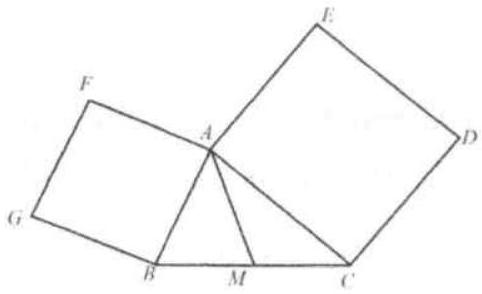
\includegraphics[width=\textwidth]{images/025(2).jpg}

Since \(B M=C M, A M=M N\), and \(\angle A M C=\angle N M B\), we have \(\triangle A M C \cong \triangle N M B\).

Thus \(B N=A C, \angle M N B=\angle M A C=\alpha\),\\
Connect \(E F\).\\
\(\angle E A F=360^{\circ}-90^{\circ}-90^{\circ}-\angle B A M-\angle M A C\)\\
\(=180^{\circ}-\beta-\alpha\).\\
\(\angle A B N=180^{\circ}-\angle B A M-\angle M N B\).\\
Since \(\angle M N B=\angle M A C=\alpha\),\\
\(\angle A B N=180^{\circ}-\angle B A M-\angle M A C==180^{\circ}-\beta\)\\
\centering
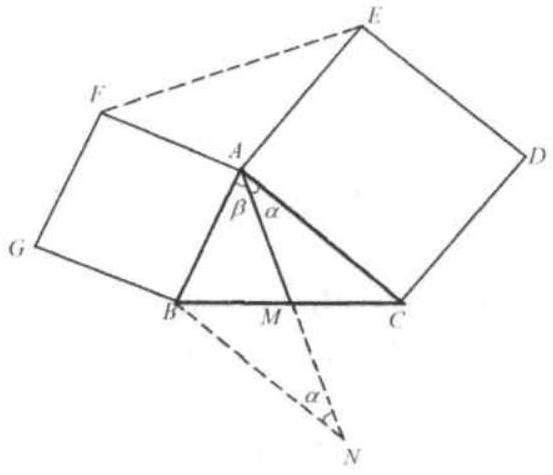
\includegraphics[width=\textwidth]{images/025.jpg}\\
\(-\alpha\).\\
Therefore, \(\angle A B N=\angle E A F\).\\
In \(\triangle E A F\) and \(\triangle N B A, A F=A B, A E=A C=B N\), and \(\angle A B N=\angle E A F\).

Thus \(\triangle E A F \cong \triangle N B A\). So \(E F=A N=2 A M\).



\end{document}
